\documentclass[11pt,a4paper]{article}
\usepackage[utf8]{inputenc}
\usepackage[T1]{fontenc}
\usepackage[brazil]{babel}
\usepackage{amsmath,amssymb}
\usepackage{graphicx}
\usepackage{geometry}
\usepackage{listings}
\geometry{margin=2.5cm}

\title{Calibração dos parâmetros $\beta$ e $\gamma$ no modelo SIR:\\
o surto de influenza de 1978}
\author{}
\date{}

\begin{document}
\maketitle

\section{Objetivo}
Este texto mostra como calibrar os parâmetros $\beta$ e $\gamma$ do modelo
SIR usando Python. O exemplo é o surto de influenza de 1978 em uma escola
interna inglesa. Usaremos os números observados ``confined to bed'' ($B$)
e ``convalescent'' ($C$), tomando
\[
 I_{\rm obs}(t_i)=B(t_i)+C(t_i)
\]
como uma aproximação observacional para o compartimento $I(t)$.

A calibração é feita por mínimos quadrados, resolvendo a EDO SIR
numericamente em cada avaliação dos parâmetros.

\section{Modelo SIR}
Para uma população fechada de tamanho $N$,
\begin{align}
S'&=-\beta SI/N,\\
I'&=\beta SI/N-\gamma I,\\
R'&=\gamma I,
\end{align}
com $S+I+R=N$. Os parâmetros têm unidade $\mathrm{dia}^{-1}$ e
\[
R_0=\frac{\beta}{\gamma},\qquad
\text{duração infecciosa média}=\frac1\gamma.
\]

\section{Dados}
Tomamos $N=763$ e as seguintes 14 observações:

\begin{center}
\begin{tabular}{c|r|r|r}
Data & $B$ & $C$ & $B+C$\\ \hline
22/01&3&0&3\\
23/01&8&0&8\\
24/01&26&0&26\\
25/01&76&0&76\\
26/01&225&9&234\\
27/01&298&17&315\\
28/01&258&105&363\\
29/01&253&162&415\\
30/01&189&176&365\\
31/01&128&166&294\\
01/02&68&150&218\\
02/02&29&85&114\\
03/02&14&47&61\\
04/02&4&20&24
\end{tabular}
\end{center}

Assim,
\[
I_{\rm obs}=(3,8,26,76,234,315,363,415,365,294,218,114,61,24).
\]

A soma $B+C$ é uma \emph{proxy} para $I$: ``convalescente'' não é
necessariamente idêntico ao compartimento infeccioso idealizado do SIR.
Por isso, os parâmetros obtidos aqui podem diferir dos parâmetros publicados
em outras análises.

\section{Condições iniciais}
Colocamos $t=0$ em 22/01 e usamos o primeiro ponto observado:
\[
I(0)=3,\qquad S(0)=760,\qquad R(0)=0.
\]

\section{Calibração}
Para cada $(\beta,\gamma)$ resolvemos a EDO e calculamos
$I(t_i;\beta,\gamma)$. Minimizamos
\[
\Phi(\beta,\gamma)=
\sum_i\left[I(t_i;\beta,\gamma)-I_{\rm obs}(t_i)\right]^2,
\qquad \beta,\gamma\geq0.
\]

O programa usa duas rotinas do SciPy.

\subsection{\texttt{odeint}}
\begin{lstlisting}[language=Python]
def sir_rhs(y, t, beta, gamma):
    S, I, R = y
    dS = -beta*S*I/N
    dI = beta*S*I/N - gamma*I
    dR = gamma*I
    return dS, dI, dR

def infected_curve(t_eval, beta, gamma):
    sol = odeint(sir_rhs, (S0,I0,R0),
                 t_eval, args=(beta,gamma))
    return sol[:,1]
\end{lstlisting}

\texttt{odeint} integra numericamente o sistema diferencial.

\subsection{\texttt{curve\_fit}}
\begin{lstlisting}[language=Python]
popt, pcov = curve_fit(
    infected_curve, t, Iobs,
    p0=(1.5,0.3),
    bounds=(0.0,np.inf),
    maxfev=20000
)
\end{lstlisting}

\texttt{curve\_fit} procura os parâmetros que minimizam a soma dos
quadrados dos resíduos. O argumento \texttt{p0} é o chute inicial e
\texttt{bounds} impõe $\beta,\gamma\geq0$.

\section{Resultado}
Para as condições e os dados acima, o ajuste dá aproximadamente
\[
\widehat\beta=1.440772\ {\rm dia}^{-1},\qquad
\widehat\gamma=0.263430\ {\rm dia}^{-1},
\]
e portanto
\[
\widehat R_0=5.469282,\qquad
1/\widehat\gamma=3.796078\ {\rm dias}.
\]
A soma dos quadrados dos resíduos é
\[
\mathrm{RSS}=20737.782747.
\]

\section{Comparação com a Figura 5-2 de White}
White apresenta, para sua análise do surto, aproximadamente
\[
\beta=1.97\ {\rm dia}^{-1},\qquad
\gamma=0.47\ {\rm dia}^{-1},
\qquad R_0=4.18.
\]
Uma nova calibração não precisa reproduzir exatamente esses valores:
as condições iniciais, a interpretação de $I$, o intervalo temporal,
a digitalização dos dados e a função objetivo podem ser diferentes.

\section{Figura}
A figura seguinte mostra os pontos $B+C$ e a curva SIR ajustada.

\begin{figure}[ht]
\centering
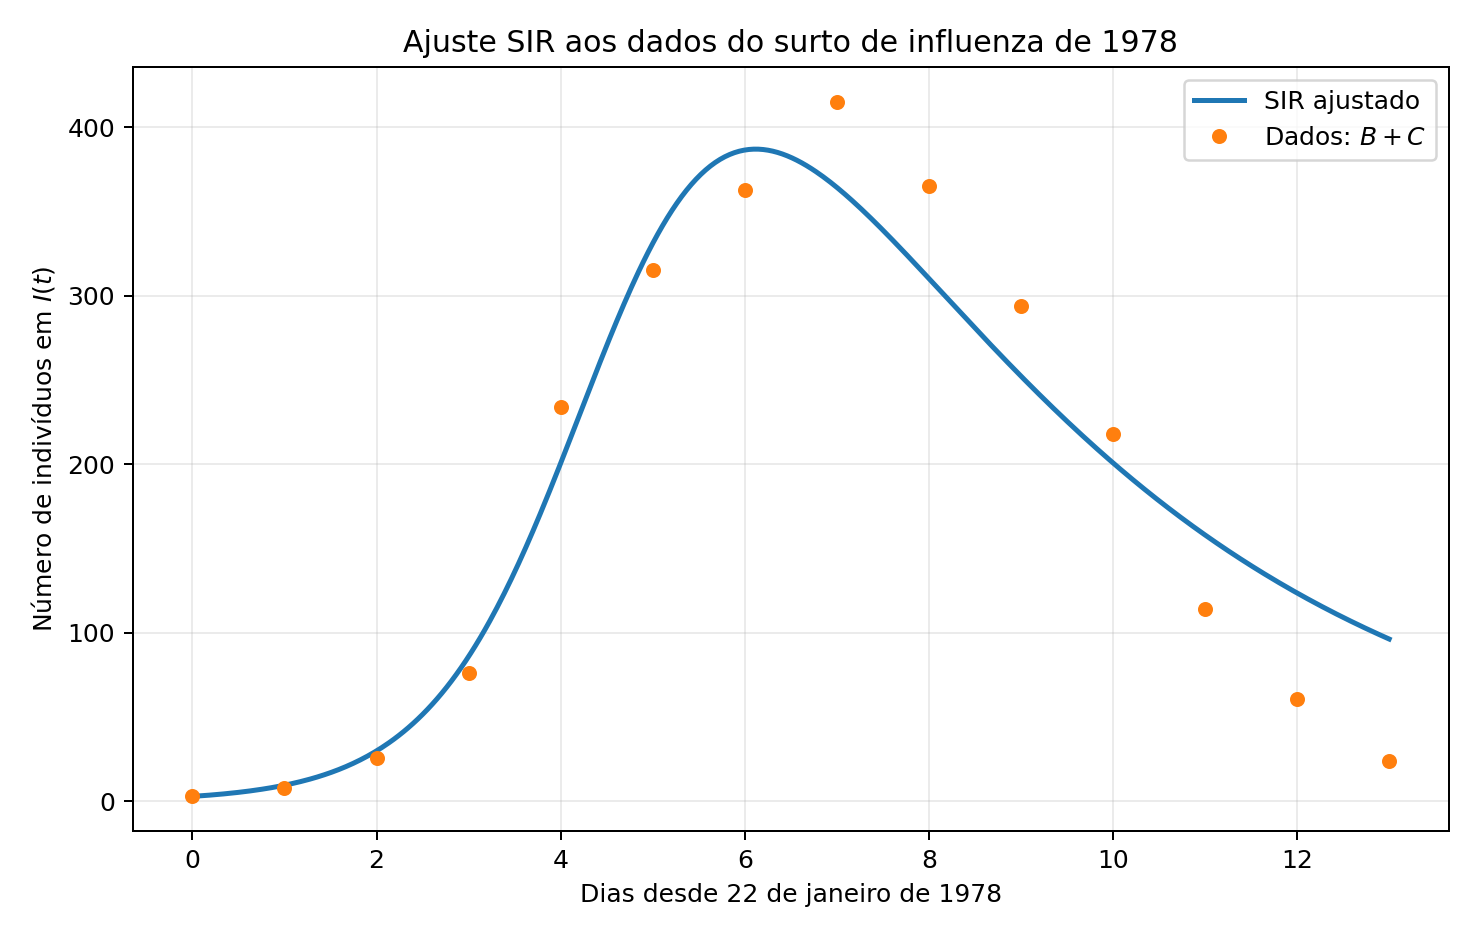
\includegraphics[width=0.90\textwidth]{calibracao_SIR_surto_BMJ_White.png}
\caption{Ajuste SIR aos dados $B+C$ do surto de influenza de 1978,
em apresentação análoga à Figura 5-2 de White.}
\end{figure}

\section{Reprodução}
Instale NumPy, SciPy e Matplotlib, por exemplo:
\begin{lstlisting}[language=bash]
pip install numpy scipy matplotlib
\end{lstlisting}
e execute:
\begin{lstlisting}[language=bash]
python calibracao_SIR_surto_BMJ_White.py
\end{lstlisting}

\section{Referências}
\begin{thebibliography}{9}

\bibitem{bmj}
``Influenza in a boarding school'', \emph{British Medical Journal},
1978.

\bibitem{white}
P. J. White, ``Mathematical Models in Infectious Disease Epidemiology'',
in \emph{Infectious Diseases}, Elsevier. A discussão inclui a aplicação
do SIR ao surto de influenza de 1978 e a Figura 5-2.

\bibitem{devries}
G. De Vries, T. Hillen, M. Lewis, J. Mueller and B. Schoenfisch,
\emph{A Course in Mathematical Biology}, SIAM, 2006.

\bibitem{scipy}
P. Virtanen et al., ``SciPy 1.0: Fundamental Algorithms for Scientific
Computing in Python'', \emph{Nature Methods} 17 (2020), 261--272,
DOI: 10.1038/s41592-019-0686-2.

\bibitem{nocedal}
J. Nocedal and S. J. Wright, \emph{Numerical Optimization}, 2nd ed.,
Springer, 2006.

\end{thebibliography}
\end{document}
